\chapter{GroundOne Studio: un'applicazione locale e un caso di studio}
\label{ch:studio}

% Source notes: Project/docs/demo_architecture.md (§13), Project/demo/docs/progress.md, Project/docs/thesis_notes.md.

I capitoli precedenti misurano GroundOne come componente isolato. Questo capitolo lo mette al lavoro dentro
un'applicazione completa, GroundOne Studio, un assistente RAG per macOS in cui recupero dei documenti, generazione della
risposta e verifica avvengono nello stesso processo, sullo stesso portatile da 16\,GB usato per gli esperimenti. L'obiettivo
è duplice. Da un lato l'applicazione completa l'argomento della località (Capitolo~\ref{sec:local}): non basta che il
verificatore possa girare in locale, serve mostrare che attorno a esso si può costruire un sistema utilizzabile senza alcun
servizio esterno. Dall'altro rende visibili, su risposte vere, le proprietà misurate nel Capitolo~\ref{sec:results}: la
verifica di tutte le frasi in un solo forward pass, le probabilità calibrate, il confronto con un giudice LLM.
Le misure raccolte nell'applicazione costituiscono un caso di studio e restano separate dai risultati del
Capitolo~\ref{sec:results}: descrivono il comportamento del sistema completo, non stabiliscono nuovi primati.

\section{Obiettivi e requisiti}
\label{sec:studio-goals}

L'applicazione è stata progettata attorno a cinque elementi che l'utente deve poter vedere, ciascuno legato a
un'affermazione della tesi (Tabella~\ref{tab:studio-requirements}). Un vincolo li accompagna tutti: nessun dato lascia la
macchina. Modelli, indice dei documenti, conversazioni e registri risiedono sul disco locale, e l'applicazione funziona
senza connessione.

\begin{table}[htbp]
\centering
\caption{Che cosa mostra l'applicazione e quale affermazione della tesi sostiene.}
\label{tab:studio-requirements}
\small
\begin{tabular}{>{\raggedright\arraybackslash}p{6.2cm}>{\raggedright\arraybackslash}p{6.8cm}}
\toprule
Che cosa vede l'utente & Affermazione sostenuta \\
\midrule
Ogni frase della risposta colorata secondo il verdetto di GroundOne, con le probabilità calibrate. & Le probabilità sono utilizzabili e coerenti con l'etichetta mostrata (RQ3). \\ \addlinespace[2pt]
Il confronto, sulla stessa risposta, con un giudice LLM eseguito localmente: verdetti e tempi affiancati. & Leggere tutti i verdetti in un solo forward pass, senza generare testo, è più accurato di un giudice LLM che scrive i verdetti, e più veloce, tanto più quanto più lunga è la risposta (RQ2). \\ \addlinespace[2pt]
Un pannello con i tempi di generazione e di verifica e la memoria occupata. & Generatore e verificatore convivono in 16\,GB, e la verifica costa poco rispetto alla generazione (RQ4). \\ \addlinespace[2pt]
La riscrittura delle frasi segnalate a partire dai documenti, verificata di nuovo. & La verifica costa abbastanza poco da stare dentro il ciclo di generazione. \\ \addlinespace[2pt]
Per ogni frase, il passaggio del documento che la sostiene o la contraddice, evidenziato. & L'attribuzione al passaggio si può ottenere con lo stesso modello; è un prototipo non valutato (Sezione~\ref{sec:concl-future}). \\
\bottomrule
\end{tabular}
\end{table}

\section{Scelte di piattaforma}
\label{sec:studio-platform}

L'applicazione è scritta in Swift, con interfaccia SwiftUI, ed esegue i modelli con MLX Swift~\cite{apple2026mlxswift,
apple2026mlxswiftlm}, la versione per Swift della stessa libreria usata per addestrare GroundOne. Sono state considerate
tre alternative: un'applicazione in Python attorno al pacchetto esistente, con interfaccia web; un'applicazione in Rust,
con collegamenti non ufficiali a MLX~\cite{oxiglade2026mlxrs} o con un altro runtime; un porting su llama.cpp con pesi
convertiti in formato GGUF. La prima avrebbe mostrato che l'esperimento può essere servito in locale, ma come server e
pagina nel browser, non come applicazione installabile. Le ultime due avrebbero richiesto di dimostrare di nuovo
l'equivalenza numerica con i risultati, e nel caso di llama.cpp di ricalibrare il modello dopo una nuova quantizzazione.
MLX Swift carica invece gli stessi pesi e lo stesso adapter e si appoggia allo stesso backend di MLX: se un test di
conformità lo conferma (Sezione~\ref{sec:studio-port}), i numeri della tesi valgono anche per l'applicazione, senza
riaddestrare né ricalibrare nulla. Il prezzo è la portabilità: l'interfaccia è legata alle piattaforme Apple, e la
compilazione degli shader di MLX richiede Xcode.

\section{Architettura}
\label{sec:studio-architecture}

L'applicazione è divisa in tre livelli (Figura~\ref{fig:studio-architecture}). Il primo è l'interfaccia. Il secondo è un
nucleo che non dipende dai motori: gestisce la sessione (risposta, verifica, riscrittura), applica la policy e salva
conversazioni e registri. Il nucleo conosce soltanto cinque interfacce astratte, dette \emph{porte}: retriever,
generatore, verificatore, giudice LLM e attributore. Il terzo livello contiene i motori che le implementano. Grazie a questa
separazione il nucleo è stato collaudato con motori fittizi, deterministici, come il pacchetto Python viene collaudato con
un backend fittizio, e un motore diverso, per esempio un generatore su llama.cpp, potrebbe sostituire quello attuale senza
toccare il resto.

\begin{figure}[htbp]
\centering
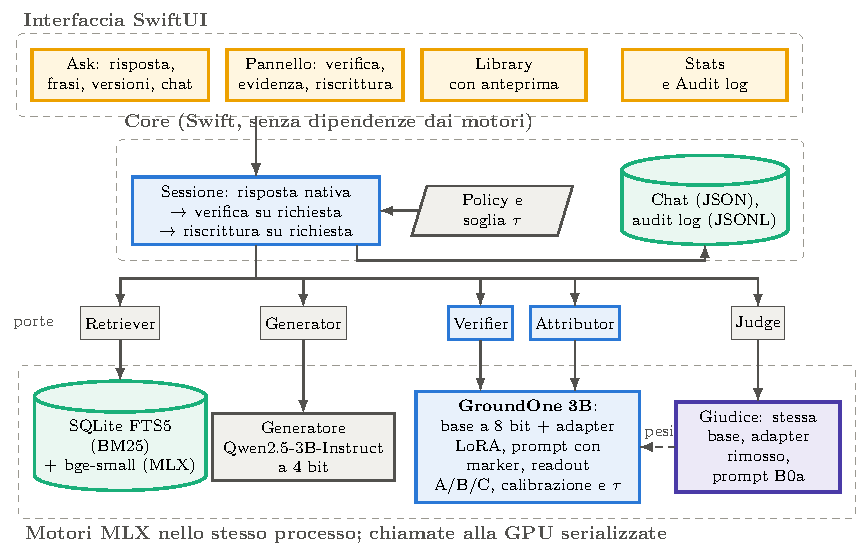
\includegraphics[width=\textwidth]{images/diagrams/studio_architecture_tikz.pdf}
\caption{Architettura di GroundOne Studio. Il nucleo conosce solo le porte; i motori, tutti nello stesso processo, sono
il retriever, il generatore, GroundOne (verificatore e, passaggio per passaggio, attributore) e il giudice LLM, che usa gli
stessi pesi di GroundOne con l'adapter rimosso. In blu le componenti in cui interviene GroundOne.}
\label{fig:studio-architecture}
\end{figure}

I motori sono quattro. Il generatore è Qwen2.5-3B-Instruct quantizzato a 4 bit, lo stesso della misura di co-residenza
della Sezione~\ref{sec:results-locality}. Il verificatore è GroundOne 3B, cioè la base a 8 bit con l'adapter LoRA, il
prompt con i marker, il readout delle lettere A, B e C e la calibrazione stimata sul dev set. È il modello predefinito
perché è il più accurato, e nell'applicazione la verifica avviene solo su richiesta, in meno di due secondi per una
risposta tipica; un selettore permette di passare al 0.5B, più rapido. Il giudice LLM del confronto è lo stesso modello base
di GroundOne con l'adapter rimosso a runtime e il prompt del giudice LLM sintetico B0a (Sezione~\ref{sec:setup-baselines}):
è esattamente il giudice LLM misurato nella tesi, non occupa memoria aggiuntiva e non lascia la macchina. Il retriever, infine,
combina un indice full-text e un piccolo modello di embedding (Sezione~\ref{sec:studio-library}).

Tutte le chiamate ai modelli passano per i contenitori dei modelli di MLX Swift, che ne serializzano l'accesso, e vengono
eseguite una alla volta sulla GPU, come avviene con il singolo thread di lavoro del servizio Python
(Sezione~\ref{sec:method-software}). Generazione e verifica non si contendono quindi le risorse, e i tempi misurati non
sono confusi da esecuzioni concorrenti. Con i tre modelli caricati, la memoria allocata da MLX è di circa 5.3\,GB e
raggiunge un picco di 6.2\,GB durante l'uso, in linea con la misura di co-residenza della
Tabella~\ref{tab:results-coresidence}, che non comprendeva il retriever. Il modello di embedding aggiunge quindi poco:
occupa circa 130\,MB su disco.

\section{Porting di GroundOne in Swift}
\label{sec:studio-port}

Quattro parti di GroundOne sono state riscritte in Swift; il resto, cioè pesi, adapter e calibrazione, viene caricato
così com'è. La prima è la costruzione del prompt. Come in addestramento, intestazione, frasi numerate, marker e a capo
vengono tokenizzati separatamente e poi concatenati, perché tokenizzare la stringa unita produrrebbe identificativi
diversi ai confini fra i pezzi. Il tokenizer è quello di swift-transformers~\cite{hf2026swifttransformers}. La seconda è il
readout: il modello calcola gli stati nascosti dell'intera sequenza, ma l'output head viene applicato solo alle posizioni
dei marker, e di ciascuna si leggono i soli logit delle tre lettere. La terza è la calibrazione: temperatura, bias e soglia
$\tau$ vengono letti dallo stesso file prodotto in Python. La quarta è la segmentazione in frasi: PySBD non esiste per
Swift, e la regola di segmentazione della Sezione~\ref{sec:data-construction} è stata riprodotta con il tokenizer di frasi
del sistema operativo~\cite{apple2026nltokenizer}, aggiungendo le stesse regole per gli elenchi e per il contenuto
verificabile.

\paragraph{Test di conformità.} Prima di costruire l'interfaccia, il porting è stato confrontato con Python su 200 risposte
di T1, stratificate per numero di frasi come il sottoinsieme usato per la latenza, per un totale di 1{,}747 marker. Python
esporta, per ogni risposta, gli identificativi dei token, le posizioni dei marker, i logit, le probabilità calibrate e le
etichette; Swift deve riprodurli (Tabella~\ref{tab:studio-conformance}). Gli identificativi dei token e le posizioni dei
marker coincidono in tutte le 200 risposte con entrambi i modelli. Con il 3B, il modello predefinito dell'applicazione, la
massima differenza tra le probabilità calibrate è 0.005 e le etichette coincidono tutte: a parità di input, i risultati
della tesi valgono quindi anche per il verificatore dell'applicazione. Con il 0.5B tre frasi su 1{,}747 superano una
differenza di 0.01, con un massimo di 0.031, e le etichette coincidono nel 99.71\,\% dei casi; ogni disaccordo riguarda
una frase la cui probabilità di supporto cade a meno di 0.01 dalla soglia. Una causa plausibile, non verificata, è un
diverso ordine delle somme in precisione ridotta, che pesa di più sul modello piccolo.

\begin{table}[htbp]
\centering
\caption{Test di conformità tra l'implementazione Swift e quella Python su 200 risposte di T1 (1{,}747 marker). I logit
sono calcolati in Swift sugli stessi identificativi dei token prodotti da Python.}
\label{tab:studio-conformance}
\small
\begin{tabular}{>{\raggedright\arraybackslash}p{6.6cm}cc}
\toprule
Controllo & GroundOne 3B & GroundOne 0.5B \\
\midrule
Identificativi dei token e posizioni dei marker identici & 200/200 & 200/200 \\
Massima differenza tra i logit & 0.070 & 0.172 \\
Massima differenza tra le probabilità calibrate & 0.005 & 0.031 \\
Frasi con differenza di probabilità sotto 0.01 & 100\,\% & 99.83\,\% \\
Etichette servite identiche & 100\,\% & 99.71\,\% \\
\bottomrule
\end{tabular}
\end{table}

Anche la velocità è quasi la stessa. Sulle stesse 200 risposte, la verifica richiede in media 2.13 secondi in Swift contro
2.04 in Python con il 3B, circa il 4\,\% in più, e 0.34 contro 0.33 secondi con il 0.5B; sono medie, mentre il
Capitolo~\ref{sec:results} riporta le mediane. La segmentazione, infine, produce le stesse frasi di PySBD nel 98.4\,\%
delle 2{,}647 risposte di T1. Le differenze residue riguardano soprattutto titoli abbreviati e citazioni che attraversano
più frasi. Senza tre regole aggiuntive, che non spezzano la frase dopo le iniziali e le abbreviazioni comuni né prima di
una parola minuscola e che uniscono i simboli di elenco alla frase seguente, l'accordo scenderebbe al 95.2\,\%.

\section{Libreria e recupero dei documenti}
\label{sec:studio-library}

La libreria dell'applicazione è formata dalle fonti di T1: i 147 articoli di cronaca CNN e Daily Mail del task di
summarization e i 450 passaggi web di MS MARCO del question answering, legati alle 150 domande reali da cui provengono. Le
schede strutturate di Yelp, in formato JSON, sono escluse, perché non sono documenti con cui conversare. I documenti
appartengono così al dominio in cui GroundOne è stato addestrato e calibrato, e le probabilità mostrate all'utente
dovrebbero conservare in buona parte il loro significato. Non è stato misurato: generatore, prompt e contesto composto da
più passaggi differiscono comunque da quelli di RAGTruth.

Ogni documento viene diviso in passaggi di circa 140 parole, allineati ai confini delle frasi, che conservano il file di
origine e la posizione nel testo. Il recupero è ibrido. Un indice full-text di SQLite~\cite{sqlite2026fts5} ordina i
passaggi con BM25\footnote{BM25 è una funzione di punteggio classica del recupero dell'informazione: premia i passaggi che
contengono i termini della domanda, pesando di più i termini rari nella collezione e attenuando l'effetto delle ripetizioni
e della lunghezza del passaggio~\cite{robertson2009bm25}.}, mentre un piccolo modello di embedding,
bge-small-en-v1.5~\cite{xiao2024cpack}, eseguito anch'esso con MLX, li ordina per similarità semantica. Le due classifiche
vengono fuse con la reciprocal rank fusion\footnote{La \emph{reciprocal rank fusion} assegna a ogni passaggio la somma,
sulle classifiche da combinare, di $1/(60 + r)$, dove $r$ è la posizione del passaggio in ciascuna classifica: un passaggio
ben piazzato in entrambe supera uno che compare in testa a una sola~\cite{cormack2009rrf}.}, e ogni documento può
contribuire con al massimo tre passaggi, così che una domanda di confronto raggiunga fonti diverse. I sei passaggi
recuperati, preceduti dalla domanda, formano il documento che GroundOne legge, nella stessa forma del question answering di
RAGTruth.

Sulle 150 domande reali di MS MARCO, il recupero ibrido riporta fra i sei passaggi tutti i passaggi originali della
domanda, con BM25 da solo come con la fusione. Il risultato è però ottimistico per costruzione: nella libreria ogni
passaggio è preceduto dalla propria domanda, usata come titolo, e la domanda posta è identica. La misura conferma che
l'indice funziona, non che il recupero sia robusto a domande formulate liberamente.

\section{L'uso dell'applicazione}
\label{sec:studio-flow}

\begin{figure}[htbp]
\centering
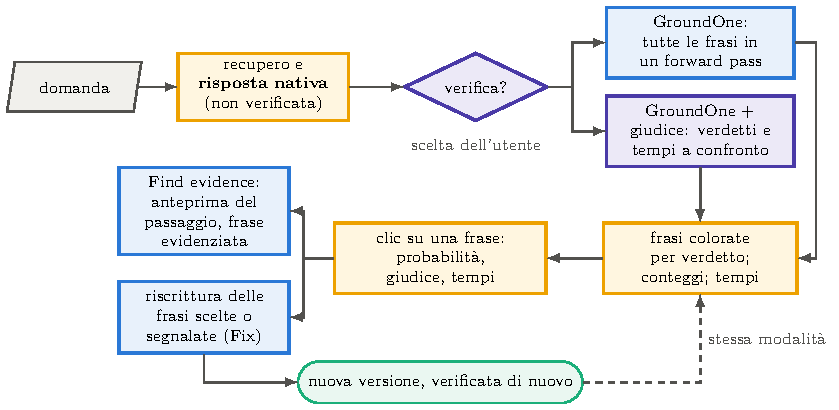
\includegraphics[width=\textwidth]{images/diagrams/studio_flow_tikz.pdf}
\caption{Il flusso d'uso. La risposta compare come l'ha scritta il generatore; la verifica, con GroundOne o con GroundOne
e il giudice LLM, e la riscrittura avvengono solo su richiesta, e ogni riscrittura produce una nuova versione verificata di
nuovo con la stessa modalità.}
\label{fig:studio-flow}
\end{figure}

Il flusso d'uso è riassunto nella Figura~\ref{fig:studio-flow}. L'utente pone una domanda, oppure sceglie uno degli esempi
proposti nella schermata iniziale. Il generatore riceve i passaggi recuperati e scrive una risposta in più paragrafi, che
compare così come è stata generata, senza alcun intervento (Figura~\ref{fig:studio-native}). Solo a questo punto l'utente
decide se verificarla, e come: con il solo GroundOne, oppure con GroundOne e il giudice LLM, per confrontare verdetti
e tempi. La separazione è voluta: mostrando per prima la risposta nativa, l'effetto della verifica resta visibile, invece di
consegnare direttamente una risposta già filtrata.

\begin{figure}[htbp]
\centering
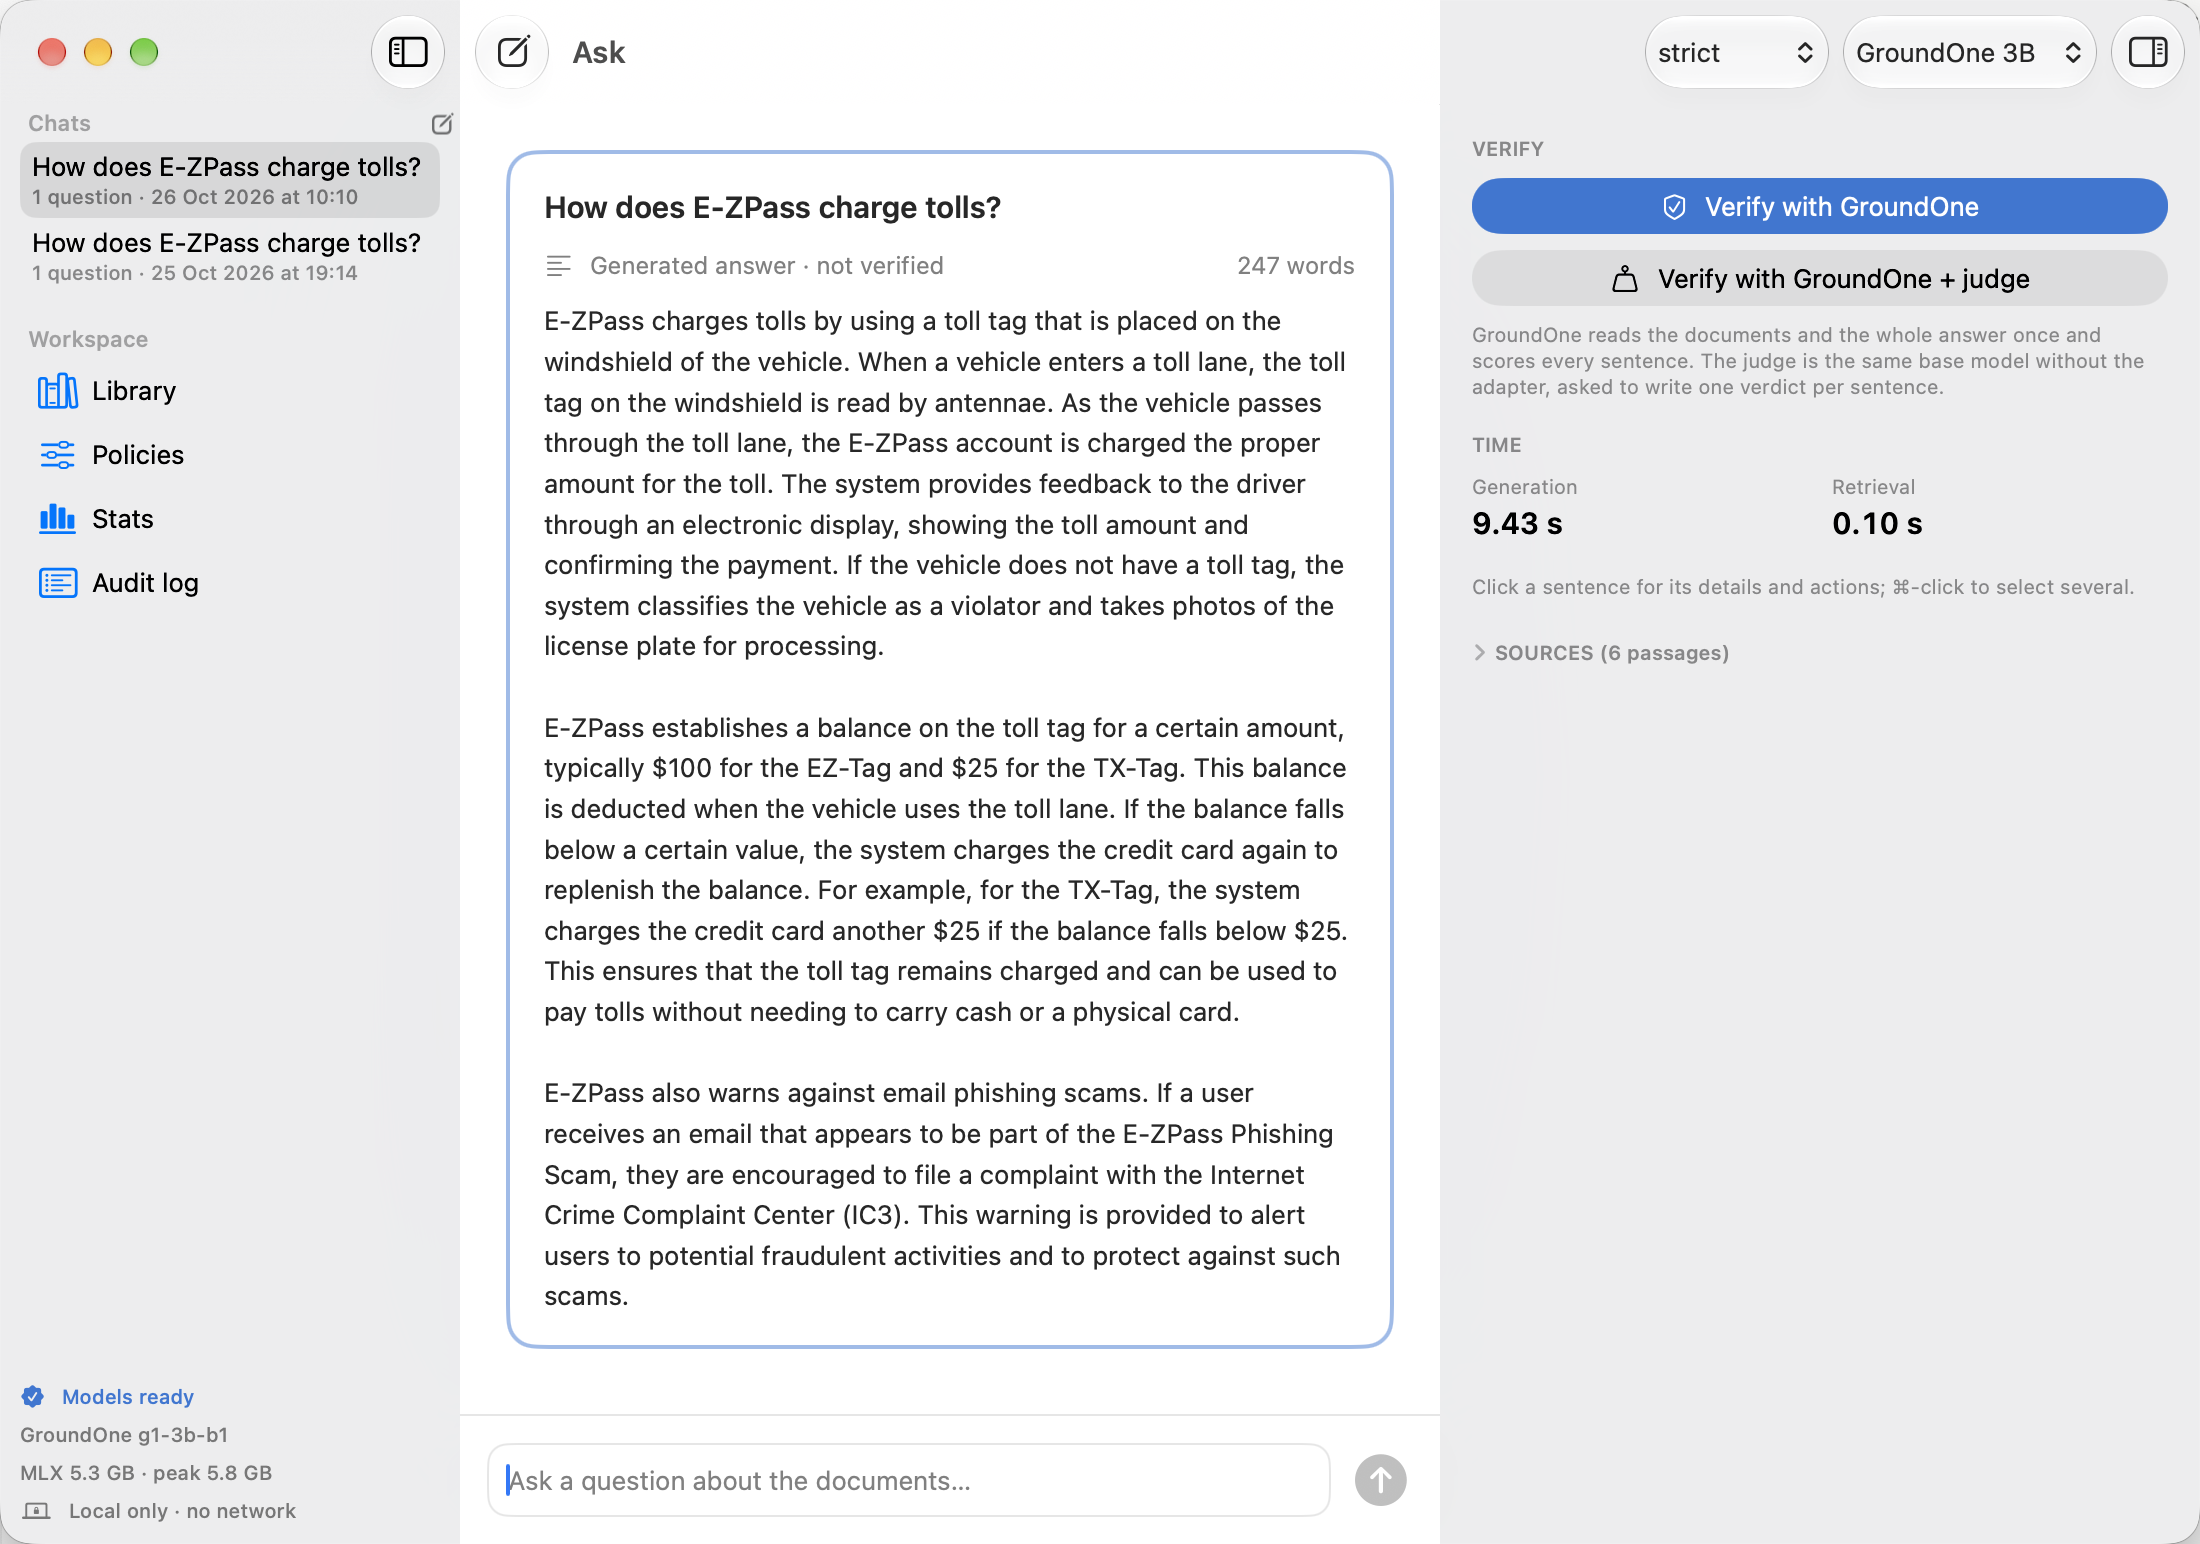
\includegraphics[width=\textwidth]{images/studio/41-native.png}
\caption{La risposta nativa del generatore alla domanda ``How does E-ZPass charge tolls?'', prima di qualunque verifica.
A destra le due modalità di verifica.}
\label{fig:studio-native}
\end{figure}

La verifica di GroundOne, in entrambe le modalità, legge l'intera risposta in un solo forward pass: tutte le frasi ricevono
il loro verdetto insieme, e una risposta con molte frasi non richiede più passaggi. Dopo la verifica le frasi si colorano:
verde tenue per le frasi supportate, rosso per quelle contraddette, arancione per quelle non menzionate dal documento; le
frasi senza contenuto verificabile restano in grigio (Figura~\ref{fig:studio-verified}). Il pannello laterale riporta i
conteggi, la soglia $\tau$, i tempi di generazione, di verifica e, se richiesto, del giudice LLM, e le frasi su cui
GroundOne e il giudice LLM non concordano.

\begin{figure}[htbp]
\centering
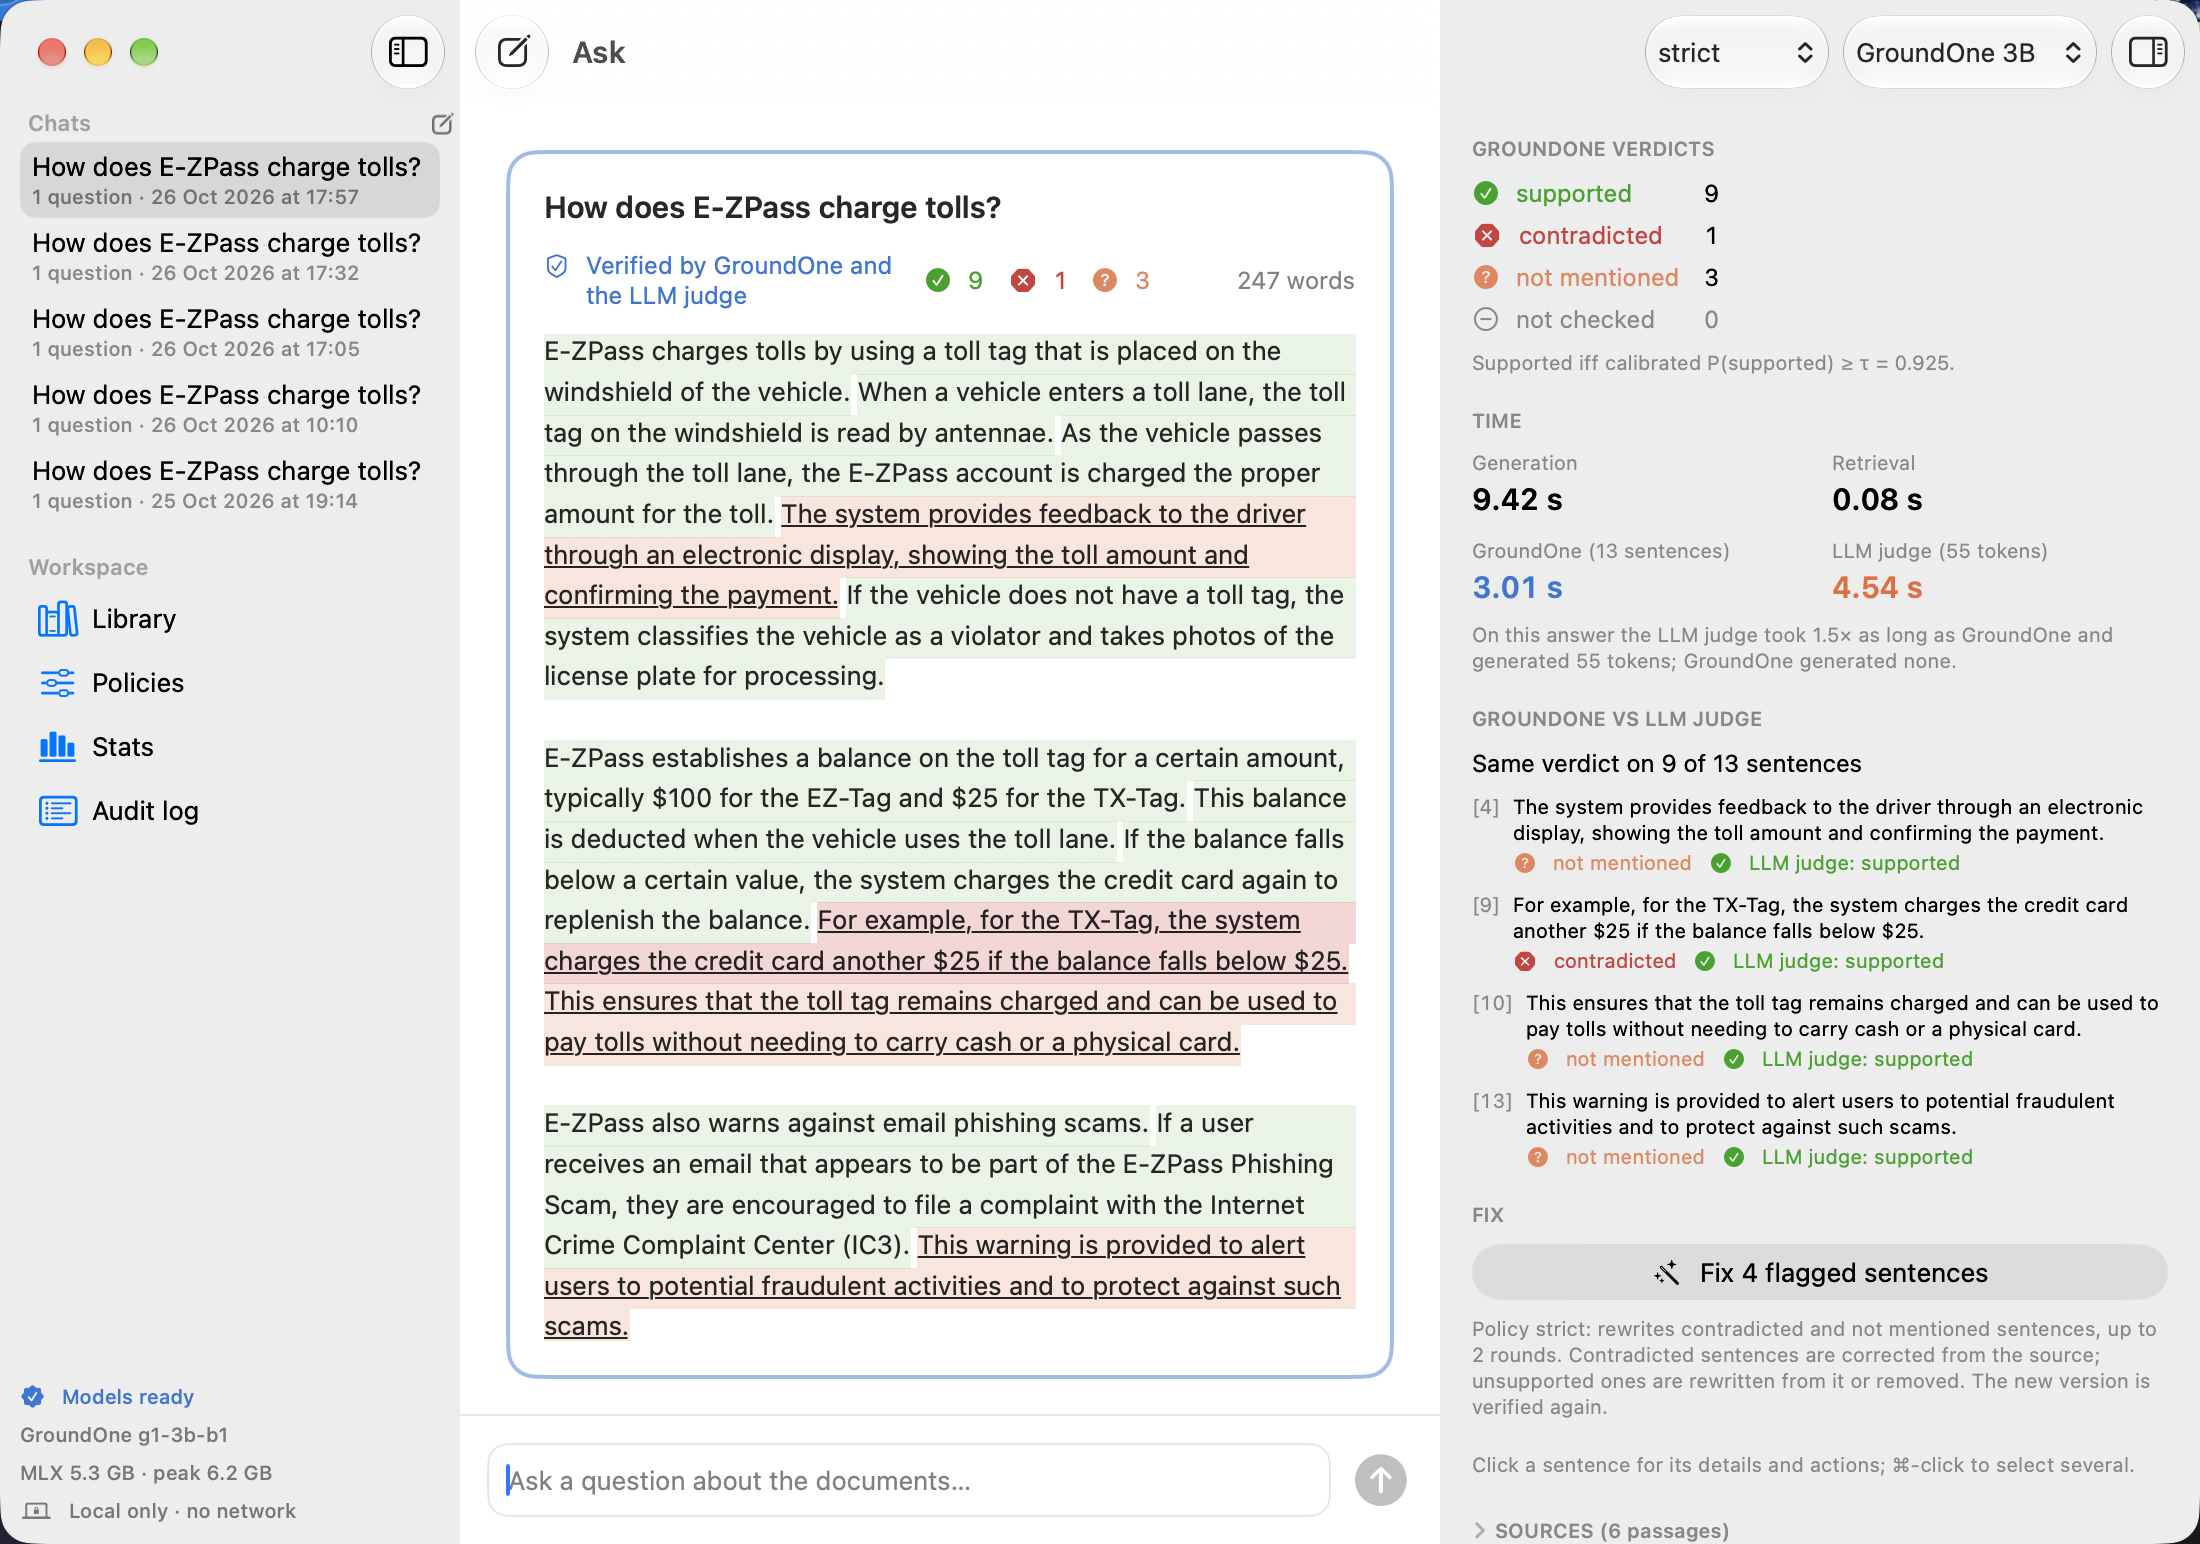
\includegraphics[width=\textwidth]{images/studio/42-verified.png}
\caption{La stessa risposta dopo la verifica con GroundOne e il giudice LLM. Le frasi sono colorate secondo il verdetto di
GroundOne; il pannello riporta conteggi, tempi e disaccordi con il giudice LLM.}
\label{fig:studio-verified}
\end{figure}

Ogni frase è selezionabile. Un clic mostra, nel pannello, le tre probabilità calibrate, il verdetto del giudice LLM e i
tempi; con il tasto Comando si possono selezionare più frasi (Figura~\ref{fig:studio-sentence}). Da qui l'utente può
chiedere l'evidenza a supporto, oppure la riscrittura delle frasi selezionate. In assenza di selezione, un pulsante
riscrive tutte le frasi segnalate secondo la policy scelta. Ogni riscrittura produce una nuova versione della risposta,
verificata di nuovo con la stessa modalità, e un selettore permette di confrontare le versioni.

\begin{figure}[htbp]
\centering
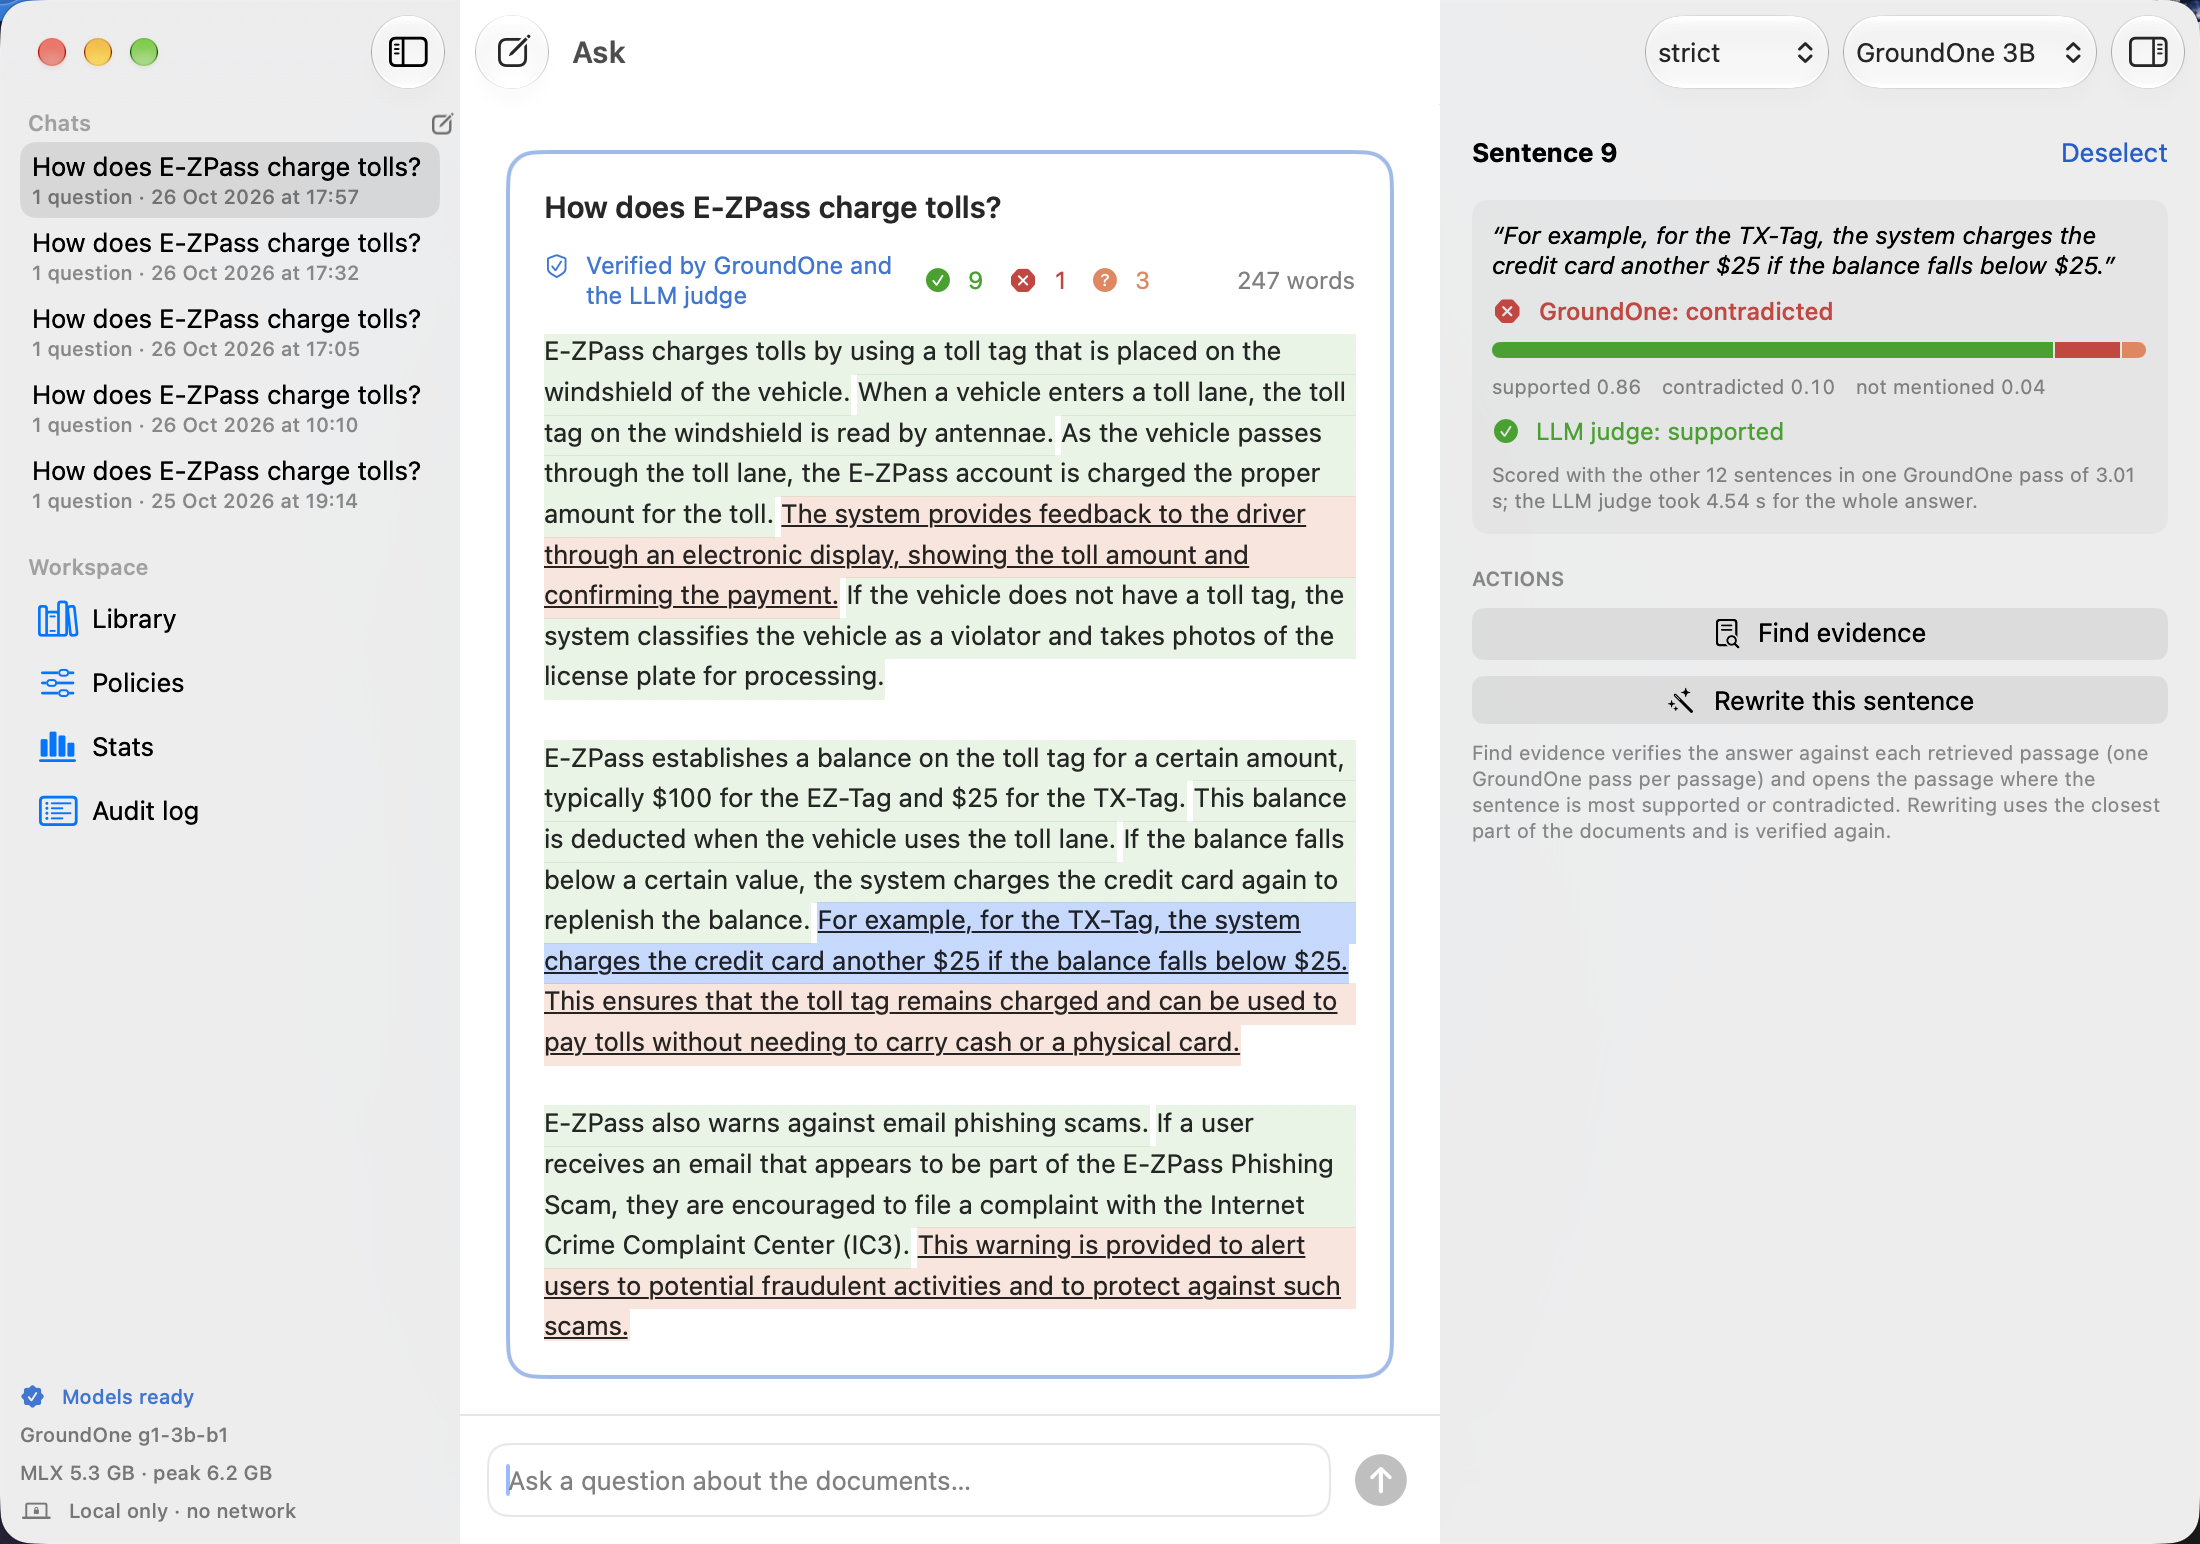
\includegraphics[width=\textwidth]{images/studio/43-sentence.png}
\caption{Il pannello di una frase selezionata: probabilità calibrate di GroundOne, verdetto del giudice LLM, tempi e azioni
disponibili.}
\label{fig:studio-sentence}
\end{figure}

\paragraph{Evidenza.} GroundOne indica se una frase è supportata, ma non da quale passaggio
(Sezione~\ref{sec:disc-limitations}). L'applicazione ricostruisce l'informazione in due passi. Nel primo verifica la
risposta contro ciascun passaggio recuperato separatamente, con un forward pass per passaggio, e sceglie quello in cui la
frase ottiene la probabilità di supporto più alta, o di contraddizione, se la frase è contraddetta. Nel secondo, dentro il
passaggio scelto, individua la frase più vicina a quella della risposta, pesando le parole condivise in base alla loro
rarità nel passaggio. L'anteprima del documento si apre con quel tratto evidenziato (Figura~\ref{fig:studio-evidence}).
È il primo prototipo del readout per passaggio indicato tra gli sviluppi futuri (Sezione~\ref{sec:concl-future}). Non è
stato valutato, perché RAGTruth non indica quale passaggio sostenga una frase, e l'applicazione lo presenta come evidenza
suggerita da GroundOne. Il calcolo avviene solo su richiesta e viene conservato: con sei passaggi costa sei forward pass,
cioè alcuni secondi con il 3B, e non modifica i tempi della verifica principale.

\begin{figure}[htbp]
\centering
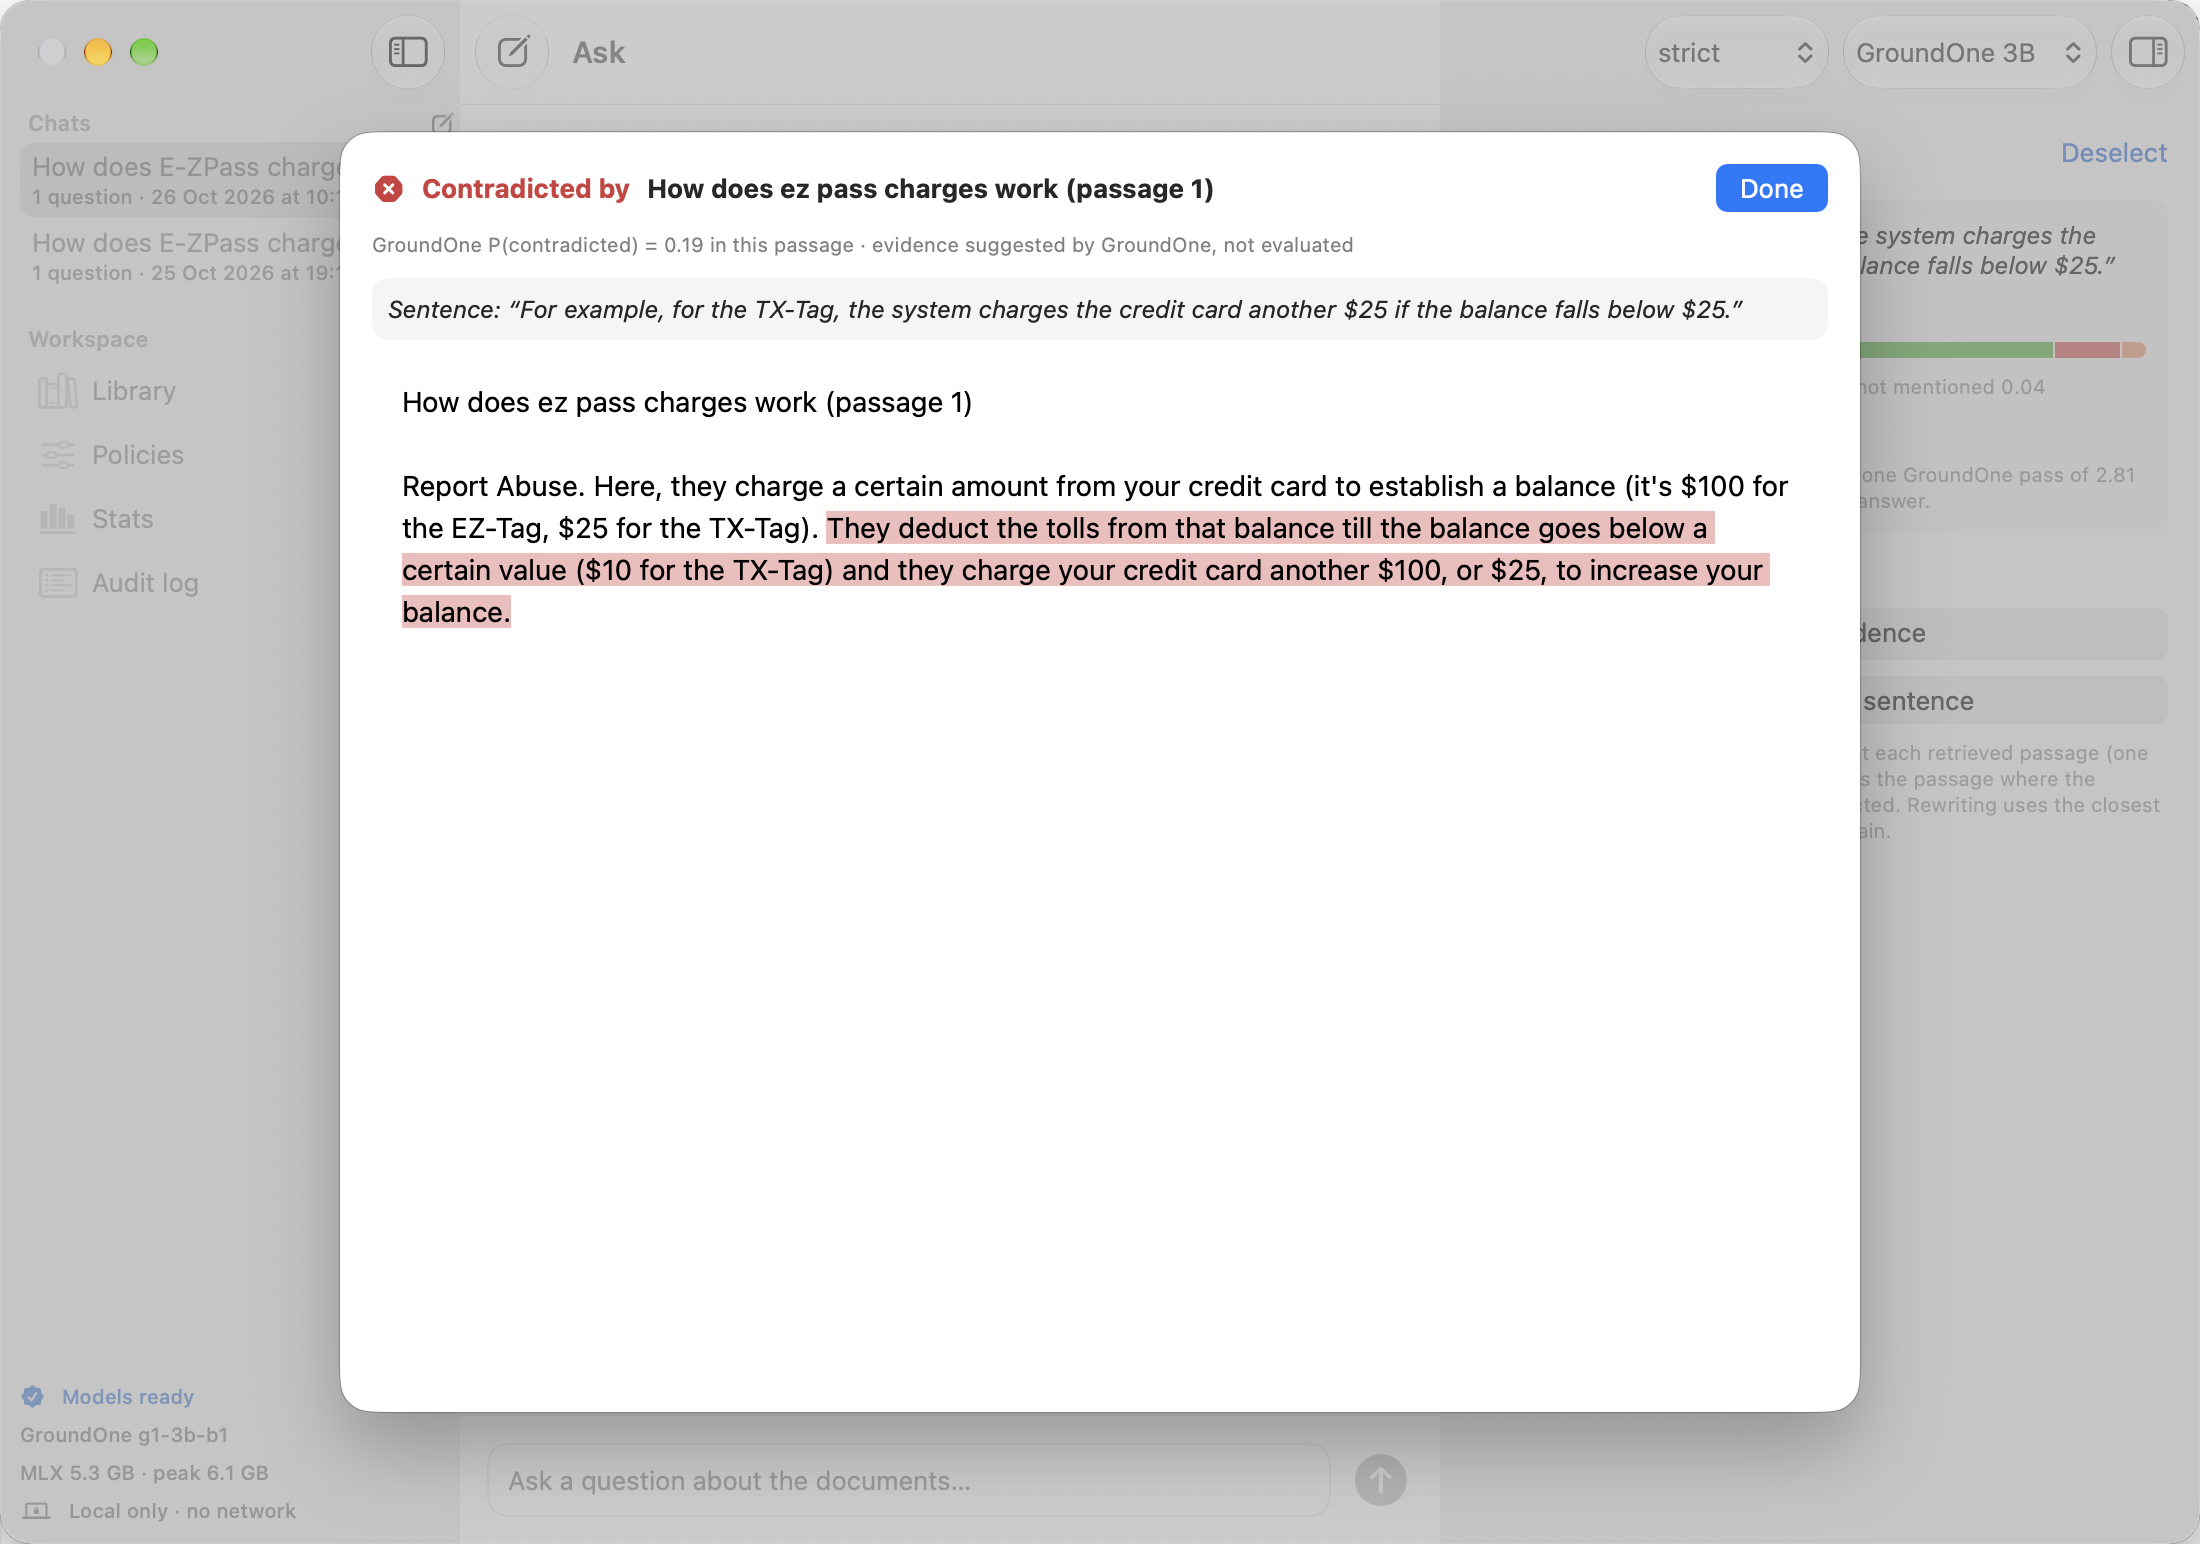
\includegraphics[width=\textwidth]{images/studio/44-evidence.png}
\caption{L'evidenza per una frase: il passaggio che, secondo GroundOne, contraddice più nettamente la frase, con il tratto
più vicino evidenziato.}
\label{fig:studio-evidence}
\end{figure}

\paragraph{Riscrittura mirata.} La riscrittura segue un principio dei cicli di verifica e revisione che si sono dimostrati
efficaci in letteratura: un critico esterno, o un'evidenza recuperata, segnala gli errori e il generatore modifica
soltanto ciò che è stato segnalato~\cite{gao2023rarr,gou2024critic}, mentre la correzione spontanea, senza un segnale
esterno, non migliora in modo affidabile le risposte~\cite{huang2024cannotselfcorrect}. GroundOne è il critico, ed è
economico: verificare di nuovo costa un solo prefill, e nemmeno completo. Le istruzioni e le fonti, già lette alla
prima verifica, restano nella KV cache (Sezione~\ref{sec:method-readout}), quindi la nuova versione richiede soltanto la
lettura della risposta riscritta, che nelle misure della Sezione~\ref{sec:results-latency-split} rende la verifica 3.4 volte più rapida con il 3B; il giudice LLM, quando è richiesto, riusa allo stesso modo la propria cache, e il
pannello dei tempi segnala quando le fonti sono state riusate. Per ogni frase da riscrivere, il generatore riceve una richiesta
breve, con la frase e il solo estratto del documento che la riguarda, e un'istruzione che dipende dal tipo di errore.
Una frase contraddetta va corretta con i fatti della fonte, e non può essere cancellata: se il generatore non restituisce
una frase utilizzabile, quella originale resta al suo posto e viene ripresentata al giro successivo. Una frase non
menzionata va riscritta con ciò che la fonte dice sullo stesso punto, oppure tolta se la fonte non ne parla. Le altre
frasi restano invariate. Il numero massimo di giri e le classi da correggere sono fissati dalla policy.

\paragraph{Policy e soglia.} Una policy è un piccolo file JSON che stabilisce quali verdetti vanno corretti, quanti giri
di riscrittura sono ammessi, che cosa fare se l'errore persiste (evidenziare, nascondere la frase o astenersi) e quale
soglia usare: quella stimata sul dev set oppure una scelta dall'utente. Le due policy predefinite corrispondono alle due
letture già introdotte nella tesi (Sezione~\ref{sec:method-calibration}): la policy strict corregge sia le frasi
contraddette sia quelle non menzionate, la policy lenient soltanto le prime.

\paragraph{Conversazioni e statistiche.} Le domande sono organizzate in conversazioni separate, che si possono
rinominare, cancellare e riprendere in qualunque momento. Una sezione dedicata raccoglie le statistiche di tutte le
verifiche eseguite nell'applicazione, anche nelle sessioni precedenti (Figura~\ref{fig:studio-stats}): il tempo di
GroundOne e quello del giudice LLM in funzione del numero di frasi, l'accordo tra i due sulle stesse frasi, la distribuzione
dei verdetti e il costo che la stessa verifica avrebbe avuto con un giudice LLM in cloud. Il costo usa gli stessi prezzi di
listino della Tabella~\ref{tab:disc-cost}: i token di ingresso sono quelli del documento e della risposta più
l'istruzione, quelli di uscita sono i token effettivamente scritti dal giudice LLM locale oppure, se il giudice LLM non è stato
eseguito, il loro numero medio per frase misurato nella tesi. Dal costo si sottrae quello dell'elettricità consumata in
locale, stimato dal tempo di verifica e dalla potenza misurata nella Sezione~\ref{sec:results-energy}.

\begin{figure}[htbp]
\centering
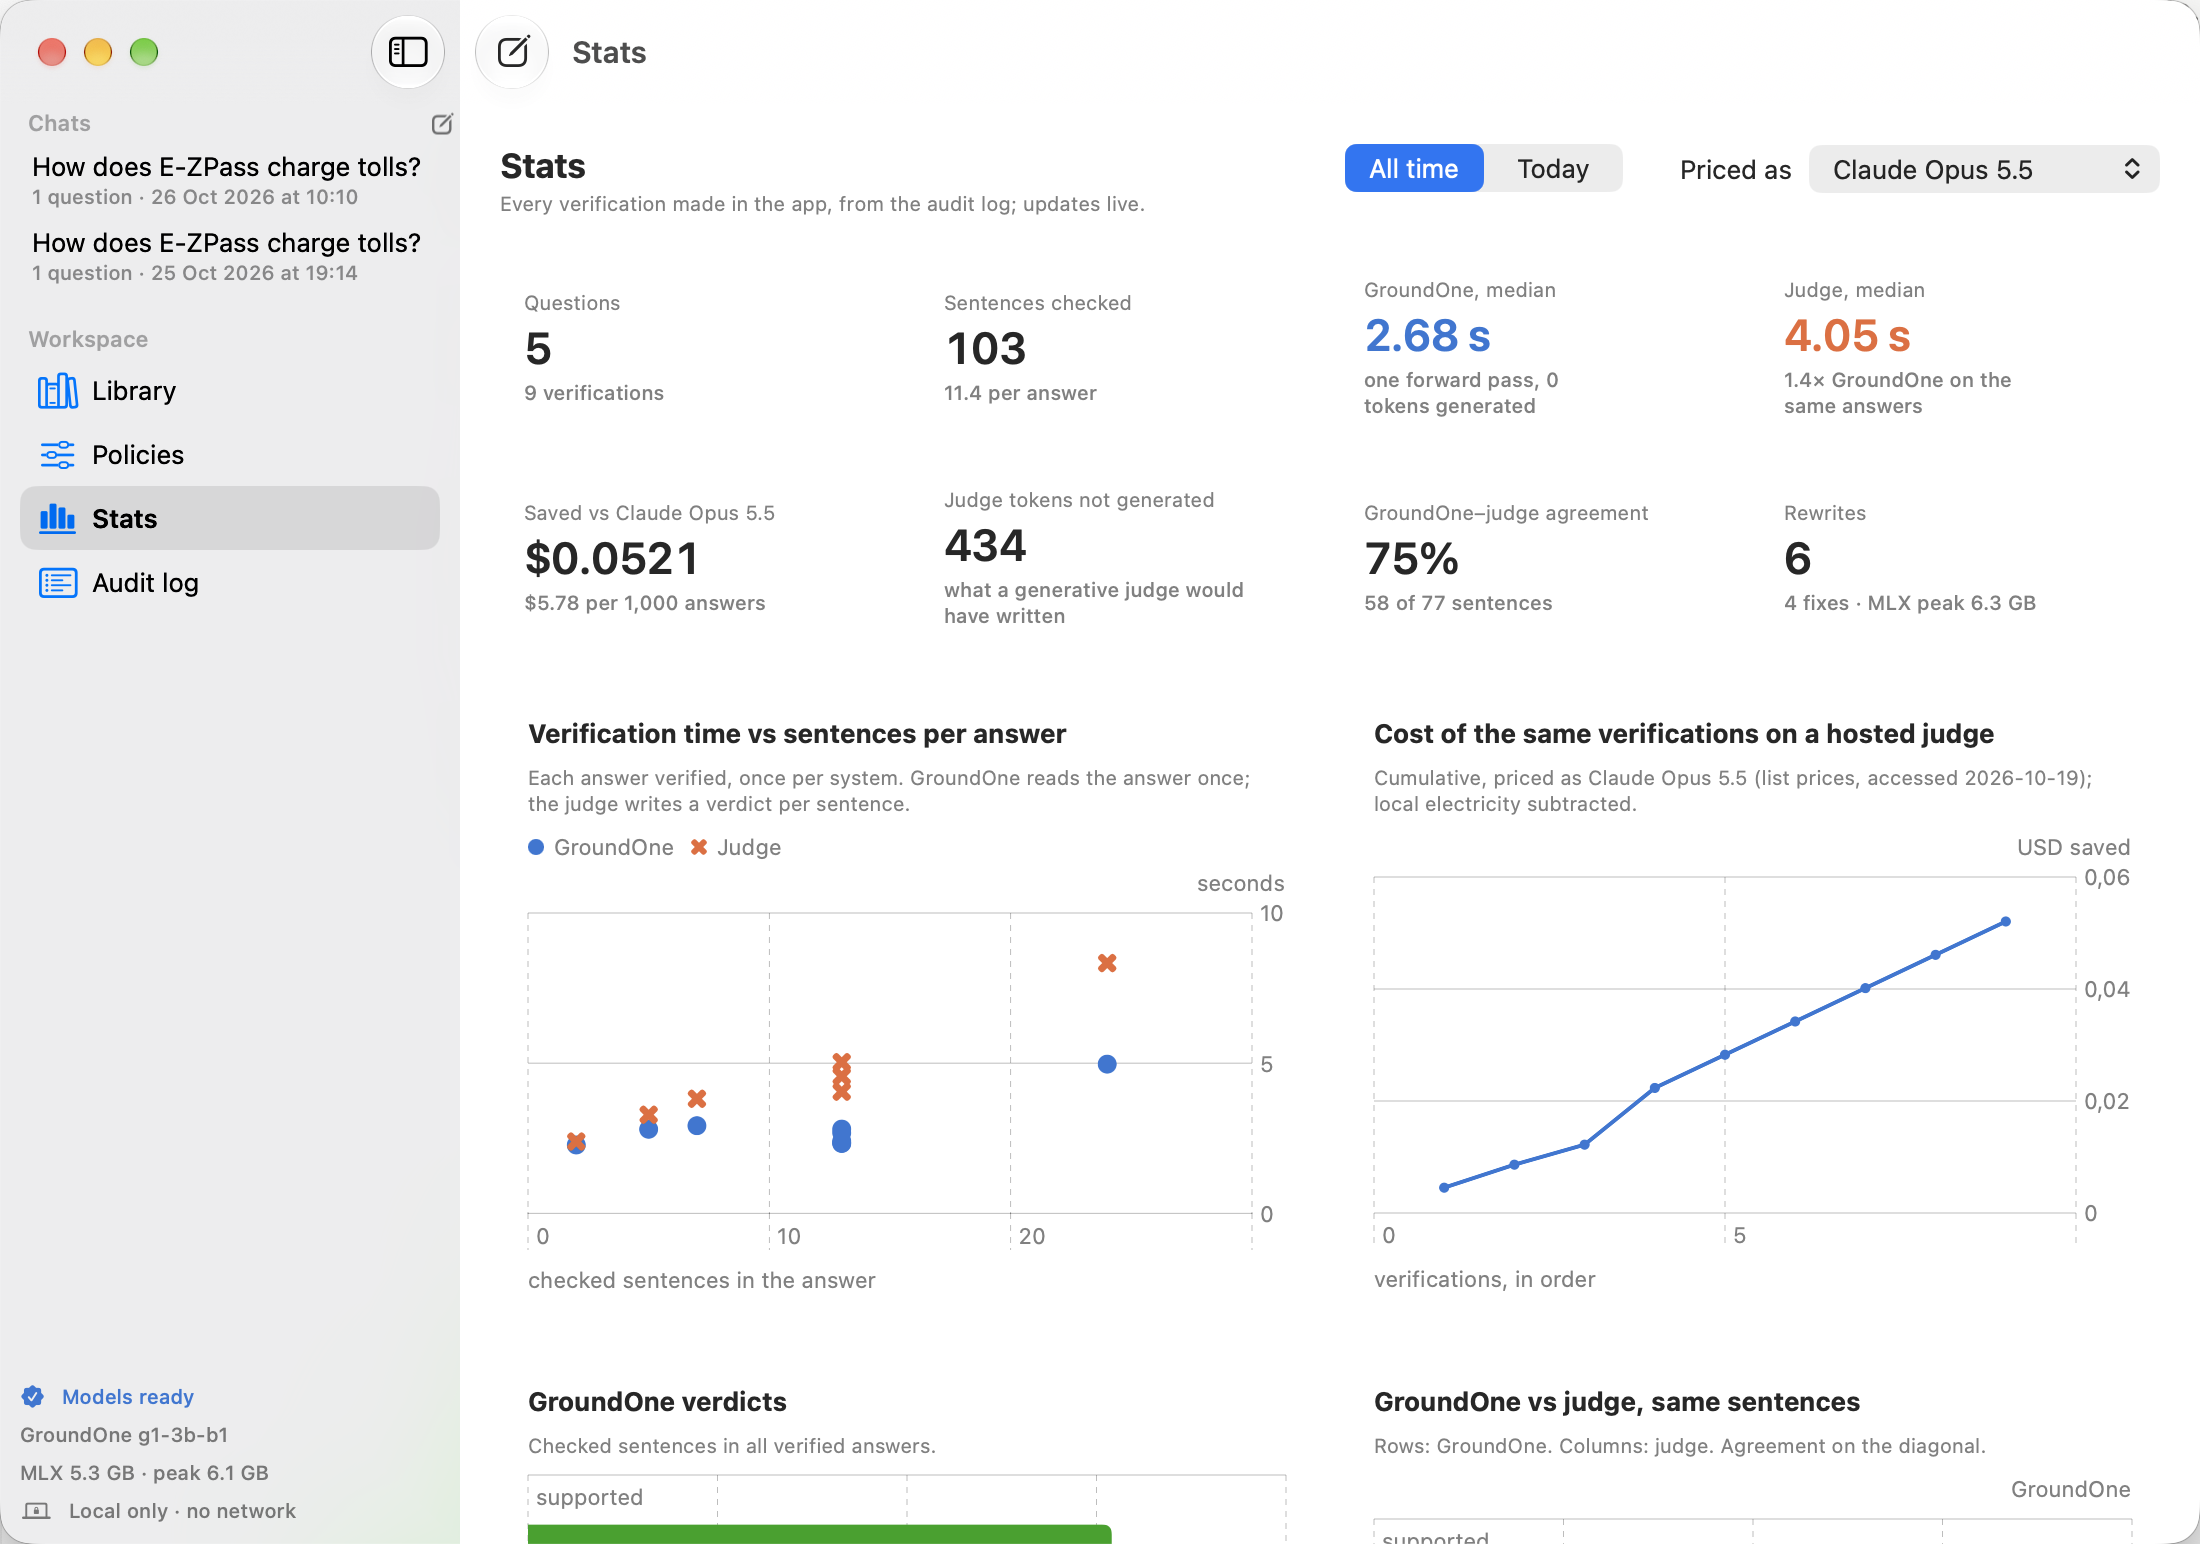
\includegraphics[width=\textwidth]{images/studio/46-stats.png}
\caption{La sezione delle statistiche: indicatori principali, tempo di verifica in funzione del numero di frasi per
GroundOne e per il giudice LLM, costo della stessa verifica su un giudice LLM in cloud.}
\label{fig:studio-stats}
\end{figure}

\paragraph{Persistenza.} Tutti i dati dell'applicazione risiedono sul disco locale, nella cartella di supporto
dell'applicazione prevista da macOS, senza alcun database server (Tabella~\ref{tab:studio-persistence}). La cartella di
supporto è stata preferita a quelle dei documenti dell'utente per una ragione pratica: macOS protegge le cartelle
Scrivania e Documenti e ne subordina l'accesso a un'autorizzazione esplicita, che un'applicazione dovrebbe chiedere
all'avvio.

\begin{table}[htbp]
\centering
\caption{Persistenza dei dati nell'applicazione. Tutto risiede sul disco locale.}
\label{tab:studio-persistence}
\small
\begin{tabular}{>{\raggedright\arraybackslash}p{3.6cm}>{\raggedright\arraybackslash}p{3.4cm}>{\raggedright\arraybackslash}p{6.0cm}}
\toprule
Dati & Formato & Uso \\
\midrule
Conversazioni & Un file JSON per conversazione. & Domande, versioni della risposta, verdetti, tempi; ripresa delle conversazioni. \\ \addlinespace[2pt]
Registro delle azioni & File JSONL in sola aggiunta. & Una riga per ogni generazione, verifica e riscrittura; base delle statistiche e del registro consultabile. \\ \addlinespace[2pt]
Libreria & Database SQLite. & Indice full-text per BM25 ed embedding dei passaggi, con l'origine di ciascun passaggio. \\ \addlinespace[2pt]
Policy & File JSON. & Regole di decisione e di riscrittura selezionabili. \\ \addlinespace[2pt]
KV cache delle fonti & Solo in memoria. & Istruzioni e ultimi documenti già letti, riusati dalle verifiche successive; non è salvata su disco. \\
\bottomrule
\end{tabular}
\end{table}

\section{Caso di studio: errori iniettati}
\label{sec:studio-casestudy}

Le risposte generate su domande libere non hanno un'etichetta di riferimento: misurare su di esse quanto il ciclo di
verifica e riscrittura migliori la risposta richiederebbe un giudizio indipendente su ogni frase riscritta. Il caso di
studio usa quindi errori iniettati, la cui posizione è nota in anticipo e non dipende da GroundOne.

\paragraph{Protocollo.} Fra le risposte di T1 le cui etichette di riferimento sono tutte ``supportata'' e che GroundOne 3B
accetta per intero, ne sono state estratte 100, dai tre task: 46 di summarization, 29 di question answering e 25 di
data-to-text. In ciascuna è stato iniettato un solo errore, di quattro tipi, 25 per tipo: un numero sostituito con un
valore assente dal documento, un nome sostituito con uno inventato, una data spostata, oppure una frase inventata inserita
dopo una frase esistente. Le risposte passano poi per lo stesso motore dell'applicazione: GroundOne verifica la risposta,
il giudice LLM la verifica a sua volta per il confronto, e la policy strict riscrive le frasi segnalate fino a due giri. Un
errore conta come rimosso quando il valore sbagliato non compare più nel testo, o quando nessuna frase resta simile a
quella inventata. Il caso di studio non usa il recupero: il documento è quello di T1.

\begin{table}[htbp]
\centering
\caption{Caso di studio sugli errori iniettati: 100 risposte di T1, un errore ciascuna, GroundOne 3B e generatore
Qwen2.5-3B-Instruct a 4 bit nello stesso processo, senza il modello di embedding. Rilevamento calcolato sulle 98 risposte
in cui la frase con l'errore riceve un proprio verdetto.}
\label{tab:studio-casestudy}
\small
\begin{tabular}{>{\raggedright\arraybackslash}p{9.4cm}c}
\toprule
Misura & Valore \\
\midrule
Frase con l'errore segnalata da GroundOne & 97 su 98 \\
Frase con l'errore segnalata dal giudice LLM & 84 su 98 \\
Falsi allarmi di GroundOne sulle altre frasi & 1.6\,\% \\
Risposte che contengono ancora l'errore: senza ciclo, dopo uno e dopo due giri & 100\,\%, 10\,\%, 9\,\% \\
Errori rimossi ripristinando il valore della fonte & 41 \\
Errori rimossi riscrivendo la frase & 1 \\
Errori rimossi cancellando la frase & 49 \\
Errori rimasti: ancora segnalati / mai segnalati & 6 / 3 \\
Altre frasi rimaste identiche & 98.2\,\% \\
Risposte accettate da GroundOne al termine & 90\,\% \\
Tempo mediano per risposta: GroundOne, giudice LLM, riscrittura per giro & 1.74\,s, 2.27\,s, 0.90\,s \\
Memoria allocata da MLX: dopo il caricamento e al picco & 5.1\,GB, 6.2\,GB \\
\bottomrule
\end{tabular}
\end{table}

\paragraph{Risultati.} La Tabella~\ref{tab:studio-casestudy} e la Figura~\ref{fig:studio-outcomes} riassumono il caso di
studio. In 98 risposte la frase con l'errore riceve un proprio verdetto; nelle altre due, il segmentatore la unisce a una
frase introduttiva priva di contenuto verificabile, e la frase non viene valutata. GroundOne segnala l'errore in 97 delle
98 risposte, il giudice LLM in 84. Il ciclo riduce le risposte che contengono ancora l'errore dal 100\,\% al 10\,\% dopo un giro
e al 9\,\% dopo due, secondo il conteggio automatico. Il modo in cui gli errori vengono rimossi conta quanto il numero. Per
i numeri e le date sostituiti, nella maggior parte dei casi il generatore ripristina il valore della fonte: 18 numeri e 16
date su 25. Le frasi inventate vengono invece cancellate, tutte e 25, ed è la correzione appropriata. I nomi inventati,
infine, sono etichettati correttamente come non menzionati, e per questo vengono per lo più tolti, 18 su 25, anziché
sostituiti con quello originale, 7 su 25: la frase perde l'errore, ma anche l'informazione. Delle nove risposte che
conservano l'errore, sei restano segnalate e vengono quindi evidenziate dalla policy. Nelle altre tre l'errore non viene mai
segnalato: in una la probabilità di supporto, 0.93, supera di poco la soglia di 0.925; nelle altre due la frase iniettata
non riceve un proprio verdetto.

\begin{figure}[htbp]
\centering
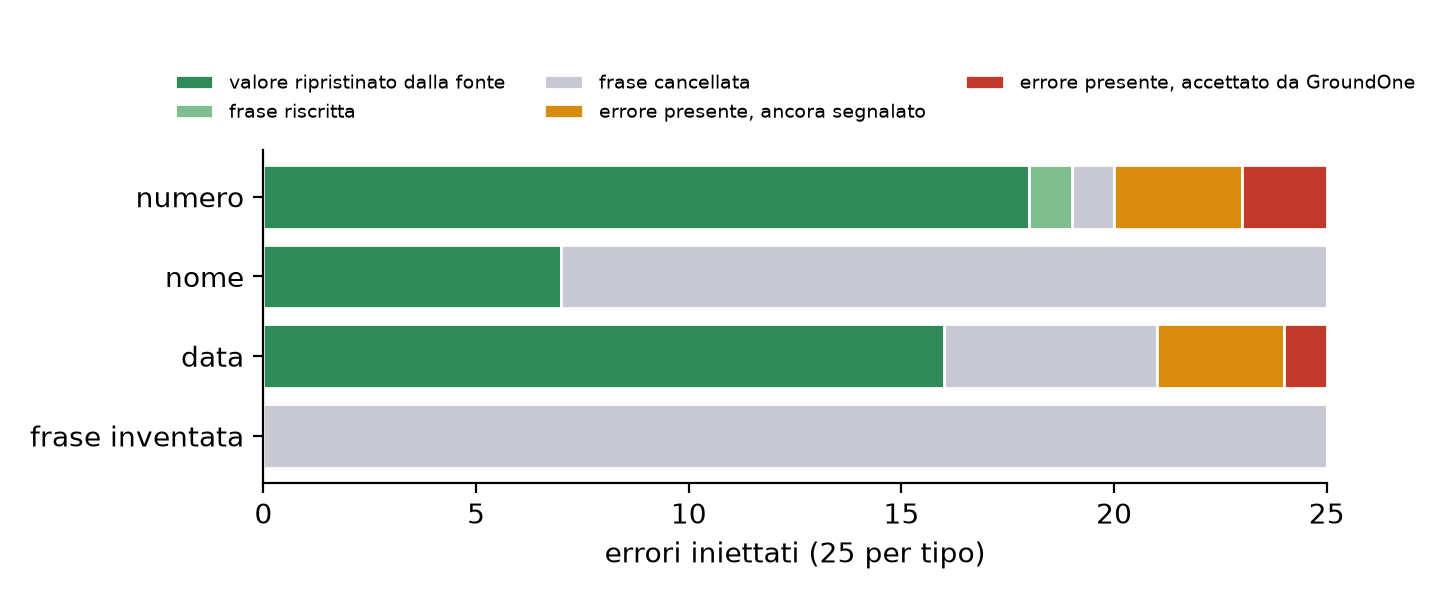
\includegraphics[width=\textwidth]{images/studio/casestudy_outcomes_g1-3b-b1-set2_it.png}
\caption{Esito di ciascun errore iniettato dopo il ciclo, per tipo di errore, con GroundOne 3B: valore ripristinato dalla
fonte, frase riscritta, frase cancellata, errore ancora presente e segnalato, errore accettato da GroundOne.}
\label{fig:studio-outcomes}
\end{figure}

\paragraph{Il tipo di errore decide la riparazione.} Ripetere il caso di studio con GroundOne 0.5B come verificatore mostra
perché il verdetto a tre classi conta, e non soltanto la segnalazione. Il 0.5B segnala l'errore in 97 risposte su 98, come
il 3B, ma etichetta quasi tutti i numeri e le date sostituiti come non menzionati (44 su 50), mentre il 3B li riconosce come
contraddetti (40 su 50). Per una frase non menzionata la riscrittura può togliere la frase, e il generatore lo fa: con il
0.5B gli errori rimossi cancellando la frase sono 87 e quelli rimossi ripristinando il valore appena 9. Le risposte che
conservano l'errore scendono al 3\,\%, ma a prezzo di informazione persa e di molti falsi allarmi: il 0.5B segnala il 17\,\%
delle altre frasi, che sono corrette, e solo l'86\,\% di esse resta invariato. La distinzione fra frase contraddetta e frase non
menzionata, che il Capitolo~\ref{sec:method} motiva in astratto, qui decide se la correzione ripristina l'informazione o
la elimina.

\paragraph{Tempi.} Il confronto dei tempi conferma il quadro della Sezione~\ref{sec:results-latency}. Su queste risposte,
con una mediana di circa 770 token tra documento e risposta e di sei frasi valutate, il tempo mediano del giudice LLM è circa
1.3 volte quello di GroundOne, e il giudice LLM scrive una ventina di token, mentre GroundOne non ne genera nessuno. La
differenza è piccola perché il giudice LLM sintetico scrive poco e le risposte sono brevi. Il confronto sul rilevamento, 97
errori segnalati contro 84, favorisce invece GroundOne per costruzione: le risposte sono state scelte fra quelle che
GroundOne accetta per intero, un filtro che il giudice LLM non ha superato, e i falsi allarmi del giudice LLM sulle frasi corrette
non sono stati misurati.

\paragraph{Un confronto a parità di calcolo.} Su 60 nuove risposte di T1, generate dal modello per ciascun task, il ciclo
completo, cioè risposta, verifica e fino a due giri di riscrittura mirata, è stato confrontato con una strategia che non
corregge nulla: generare fino a tre risposte con campionamento e tenere la prima che GroundOne accetta. La prima risposta
è accettata nel 52\,\% dei casi. Al termine, il ciclo porta le risposte accettate al 63\,\%, la generazione multipla al
62\,\%; il ciclo impiega però una mediana di 6.9 secondi e 115 token generati, contro 10.3 secondi e 218 token. Le
riscritture, quindi, non accettano più risposte di quante ne accetterebbe rigenerarle da capo, ma costano circa due terzi
del tempo e la metà dei token. Una parte delle risposte resta segnalata perché il generatore da 3B non riesce a correggere
una frase contraddetta, che il ciclo non può cancellare.

\paragraph{Come leggere i risultati.} Tre avvertenze delimitano la portata del caso di studio. La prima riguarda il
rilevamento. Le risposte sono state scelte fra quelle che GroundOne accetta, e gli errori iniettati sono netti: valori e
nomi assenti dal documento. L'alta percentuale di errori segnalati mostra quindi il funzionamento del ciclo, non la
recall di GroundOne, che è misurata nel Capitolo~\ref{sec:results}. La seconda riguarda le frasi riscritte: non hanno
un'etichetta di riferimento, e la loro correttezza è giudicata soltanto da GroundOne, lo stesso modello che decide quando
fermare il ciclo. Una riscrittura che cade in un punto cieco del modello viene quindi contata come riuscita, e il conteggio
automatico registra soltanto la scomparsa dell'errore iniettato, non eventuali nuovi errori introdotti dalla riscrittura.
Per questo i risultati sono espressi come risposte ``accettate da GroundOne'', non come risposte corrette, e il 90\,\% di
risposte accettate comprende tre risposte che contengono ancora l'errore. La terza riguarda il generatore. Un modello da 3B
a volte non sa correggere una frase e a volte la toglie: 24 dei 49 errori rimossi per cancellazione portano via anche
un'informazione corretta, per cui una parte delle risposte accettate è semplicemente più breve.

\section{Un esempio: un errore numerico sottile}
\label{sec:studio-example}

La domanda della Figura~\ref{fig:studio-native} mostra in piccolo sia il valore sia i limiti del sistema. Fra le tredici
frasi della risposta, il generatore scrive che, per la tessera TX-Tag, la carta di credito viene ricaricata di 25 dollari
quando il saldo scende sotto i 25 dollari. Il passaggio recuperato dice invece che la ricarica avviene quando il saldo
scende sotto i 10 dollari. La frase ricalca la fonte quasi parola per parola, ed è proprio il tipo di errore che la
Sezione~\ref{sec:results-errors} indica come il più difficile per GroundOne. GroundOne le assegna una probabilità di
supporto di 0.86, sotto la soglia di 0.925, e indica la contraddizione come errore più probabile; il giudice LLM
la considera supportata. GroundOne segnala inoltre come non menzionate tre frasi che aggiungono dettagli o deduzioni
assenti dai documenti, per esempio che il display mostri l'importo del pedaggio, mentre il giudice LLM le accetta tutte.
La riscrittura, però, non riesce: il generatore da 3B restituisce la stessa frase, con lo stesso importo sbagliato, a
conferma che la qualità del ciclo dipende anche dal generatore.

\section{Probabilità calibrate e soglia di decisione}
\label{sec:studio-threshold}

L'esempio aiuta a chiarire un punto che l'uso dell'applicazione rende evidente. Le probabilità di GroundOne sono
calibrate: su T1, fra le frasi a cui il 3B assegna una probabilità di supporto compresa tra 0.80 e 0.925, il 93\,\% è
effettivamente supportato. Eppure tutte queste frasi vengono segnalate, perché la soglia è 0.925. Le due cose non sono in
contraddizione. La calibrazione riguarda il significato delle probabilità; la soglia è una regola di decisione, scelta sul
dev set per massimizzare la balanced accuracy a tre classi (Sezione~\ref{sec:method-calibration}). Poiché la grande
maggioranza delle frasi è supportata, circa l'88\,\% nel dev set e il 91\,\% in T1, una metrica che pesa allo stesso modo
le tre classi spinge la soglia verso l'alto: per trovare gli errori, rari, accetta molti falsi allarmi
(Tabella~\ref{tab:studio-threshold}).

\begin{table}[htbp]
\centering
\caption{Effetto della soglia sulle frasi di T1 con GroundOne 3B: quota di frasi segnalate e recall per classe.}
\label{tab:studio-threshold}
\small
\begin{tabular}{cccccc}
\toprule
$\tau$ & \makecell{Frasi\\segnalate} & \makecell{Recall\\supportate} & \makecell{Recall\\contraddette} & \makecell{Recall\\non menzionate} & \makecell{Balanced\\accuracy} \\
\midrule
0.5 & 7\,\% & 0.98 & 0.56 & 0.60 & 0.71 \\
0.8 & 15\,\% & 0.92 & 0.71 & 0.83 & 0.82 \\
0.925 & 25\,\% & 0.82 & 0.78 & 0.89 & 0.83 \\
\bottomrule
\end{tabular}
\end{table}

Passare da 0.8 a 0.925 aggiunge appena 0.01 di balanced accuracy, ma porta le frasi segnalate dal 15\,\% al 25\,\%, quando
gli errori veri in T1 sono il 9\,\%. D'altra parte, l'errore sulla tessera TX-Tag sta proprio in questa fascia: con una
soglia di 0.8 sarebbe passato inosservato. Il caso di studio offre l'esempio speculare: l'unico errore che GroundOne lascia
passare ha una probabilità di supporto di 0.93, appena sopra la soglia. Nessuna delle due scelte è sbagliata. Una soglia
alta conviene quando un errore non segnalato costa molto, una soglia più bassa quando i falsi allarmi disturbano l'utente.
È questo il vantaggio pratico delle probabilità calibrate: la soglia si può scegliere in modo consapevole, e l'applicazione
la espone come parametro della policy. L'etichetta mostrata per una frase sotto soglia va letta di conseguenza: indica il
tipo di errore più probabile, non una certezza, ed è per questo che il pannello riporta sempre le tre probabilità.

\section{Limiti}
\label{sec:studio-limits}

\paragraph{Il generatore.} Il generatore da 3B scrive risposte più brevi di quanto richiesto, fra circa 120 e 250 parole
contro le 300--500 indicate nel prompt, e non sempre riesce a correggere una frase segnalata: nell'esempio della
Sezione~\ref{sec:studio-example} restituisce la frase invariata. Un generatore più grande, per esempio da 7B a 4 bit,
starebbe ancora nella memoria del portatile e dovrebbe migliorare entrambi gli aspetti, ma non è stato valutato.

\paragraph{Le frasi riscritte.} La correttezza delle frasi riscritte è giudicata solo da GroundOne. Un controllo
indipendente, con un secondo verificatore come un encoder specializzato oppure con una lettura umana di un campione,
permetterebbe di misurare quante riscritture accettate siano davvero corrette.

\paragraph{L'evidenza.} L'evidenza suggerita non è stata valutata, perché i dati non indicano quale passaggio sostenga
ciascuna frase. È una funzione dimostrativa.

\paragraph{Ambito.} L'applicazione eredita i limiti di GroundOne (Sezione~\ref{sec:disc-limitations}): verifica documenti
e risposte in inglese, nel dominio dei dati di addestramento, e si basa sui documenti recuperati, non sulla verità del
mondo. Domande che riguardano l'intera libreria, per esempio una panoramica dei documenti, non sono alla portata di un
sistema che recupera sei passaggi. L'interfaccia, infine, gira soltanto su macOS, e il generatore e il verificatore 3B
sono soggetti alla licenza di Qwen per la ricerca (Sezione~\ref{sec:setup-licences}): l'applicazione è un prototipo di
ricerca, non un prodotto.
